

\chapter{Numerical Optimization}
\label{numerics}

\section{Floating Point Calculations}

\section{Newton's Method}

\section{Gradient Based Optimization}
\label{gradient-optimization}

\subsection{More on Gradient Descent}
\label{gradient descent}
Suppose that we let $\vec{x}_0\in \R^n$ to be our starting condition,
$g=\triangledown_x f(\vec{x_0})$, and $f: \R^n\rightarrow\R$.
Our goal is to use gradient descent to minimize $f(\vec{x_0})$.

Thus we have the Hessian: $H=H(f)(\vec{x_0})$, and a direction to step in:  $\hat{u}=\frac{\vec{x}-\vec{x_0}}{||\vec{x}-\vec{x_0}||_2}$. Then $f(\vec{x})\approx f(\vec{x_0})+(\vec{x}-\vec{x_0})^T\vec{g}+\frac{1}{2}(\vec{x}-\vec{x_0})^TH(\vec{x}-\vec{x_0})$. Note that this is only accurate locally. In other words, $f(\vec{x})$ is the composition of the initial condition, the gradient (first derivative) in direction $\vec{x}-\vec{x_0}$, and the Hessian (second derivative) in direction $\vec{x}-\vec{x_0}$.

\begin{definition}
Gradient Descent Step\\
Consider $\vec{x}$ as a combination of the initial position with a step in a certain direction. Let $\alpha$ be the step and $\vec{g}$ be the direction.
Thus $f(x_0-\alpha\vec{g})\approx f(x_0)-\alpha \vec{g}^T\vec{g}+\frac{1}{2}\alpha^2\vec{g}^TH\vec{g}$ Assuming the Hessian is not zero there are 2 cases.\\
Case 1: Suppose $f$ is positive definite. That implies that $\vec{g}^TH\vec{g}>0$. Then to compute the optimal step size find where the derivative is 0:
\begin{align*}
    \frac{d}{d\alpha}f(\vec{x_0}-\alpha \vec{g})=-\vec{g}^T\vec{g}+\alpha\vec{g}^TH\vec{g}\\
    \Longrightarrow \alpha=\frac{\vec{g}^T\vec{g}}{\vec{g}^TH\vec{g}}
\end{align*}\\
Case 2: Suppose $\vec{g}^TH\vec{g}<0$. Then, by Taylor series, this will cause $f(\vec{x})$ decrease forever. (Note that this is probably not always the case since this approximation is only accurate locally)\\
\end{definition}

Thus by finding what direction $\vec{g}$ the gradient is changing in, we can eventually find the extrema of $f(\vec{x})$

Recall, the 2nd Derivative Test for convexity from your calculus test, similarly we have the 2nd Derivative Test with Hessians.
\begin{theorem}
2nd Derivative Test\\
Suppose $\triangledown_{\vec{x}} f(x)=\vec{0}$\\
\begin{enumerate}
    \item If $H(f)(\vec{x_0})$ is positive definite, meaning $\vec{g}^TH\vec{g}>0$, the $\vec{x_0}$ is a local minimum.
    \item If $H(f)(\vec{x_0})$ is negative definite, meaning $\vec{g}^TH\vec{g}<0$, the $\vec{x_0}$ is a local maximum.
    \item If $H(f)(\vec{x_0})$ has negative and positive eigenvalues, meaning $H$ is increasing and decreasing give different directions, the $\vec{x_0}$ is a saddle point.
\end{enumerate}
\end{theorem}
\begin{remark}
The condition number $\max\limits_{i,j} \lvert\frac{\lambda_i}{\lambda_j} \rvert$
of H indicates how well a gradient descent step will preform. Specifically a large condition number would imply that the gradient step will over step. 
\end{remark} 

\begin{example}
Suppose in 2D $H(f)=
\begin{pmatrix} 
10 & 0\\
0 & 1
\end{pmatrix}
$
\end{example}
The issue here is...
\underline{Fixes:}
\begin{enumerate}
    \item Use the Hessian in the algorithm
    \item Normalize the data (similar to the change of variables which makes the level curves more circle; Hint: Logical Regression)
\end{enumerate}
So, when can we guarantee that gradient descent or some variation with converge? -> in deep learning this will never happen.


\subsection{Gradient Descent Convergence}
\label{GD-convergence}

How can we guarantee that gradient descent converges? It is impossible to guarantee for all functions. But for a specific class of functions, using \cvx{} optimization, we can provide such a theorem:

\begin{theorem}[Gradient Descent Guarentee]
    Suppose that $f : \R^n \rightarrow \R$ is twice differentiable, \cvx, whose gradint is $\Lip$-Lipschitz continuous, and has a global minimum $\vx^* \in \R^n$. 
    If $\vx_{k}$ is the $k^{th}$ step of gradient descent with fixed step size $\alpha < \frac{1}{L}$, and $\vx_0$ is the initialization point, then we have
    $$f(\vx_k) - f(\vx^*) \leq \frac{\norm{\vx_0 - \vx^*}_2^2}{2\alpha k}$$
\end{theorem}

\begin{remark}
    By choosing $k$ large enough (performing several gradient descent steps), we can make $\frac{\norm{\vx_0 - \vx^*}_2^2}{2\alpha k}$ as small as necessary (as everything else in this expression is constant). That means that by going far enough in gradient descent, it is possible to guarentee that the value of $f(\vx_k)$ is within any desired distance from the global minimum.
\end{remark}

\begin{proof}

    \label{proof-theoreme-gd-converge}
    First, we need to use the fact that the gradient $\nabla_\vx f(\vx)$ is $\Lip$-Lipschitz continuous implies that $H(f)(\vx) - \Lip I$ is negative semi-definite. To prove this fact, let's introduce some notation. Let $f : \R \rightarrow \R, f_{\vx,\vuhat}(t) = f(\vx + t\vuhat),   \forall \vx,\vuhat \in \R^n$ where $\vuhat$ is a unit vector. Then we have its derivative in $t=0$ equal to $f'_{\vx,\vuhat}(0) = \vuhat^T \nabla_\vx f(\vx)$ which is the directional derivative in the direction of $\vuhat^T$. With this, we can show that $H(f)(\vx) - \Lip I$ is negative semi-definite by proving that $\vuhat^T(H(f)(\vx) - \Lip I) \vuhat$ is always lesser than or equal to 0:
    \begin{ceqn}
        \begin{align*}
            \vuhat^T(H(f)(\vx) - \Lip I) \vuhat &= \vuhat^T H(f)(\vx)\vuhat - \vuhat^T \Lip I \vuhat \\
            &= \vuhat^T H(f)(\vx)\vuhat - \Lip
        \end{align*}
    \end{ceqn}
    Here, $\vuhat^T H(f)(\vx)\vuhat$ is the second derivative of $f$ in direction of $\vuhat$. So this expression is actually equal to $f''_{\vx,\vuhat}(0) - \Lip$ and we can write 
    \begin{ceqn}
        \begin{align*}
            \vuhat^T(H(f)(\vx) - \Lip I) \vuhat &= f''_{\vx,\vuhat}(0) - \Lip \\
            &= \lim_{h \to 0} \frac{f'_{\vx,\vuhat}(h + 0) - f'_{\vx,\vuhat}(0)}{h} - \Lip \\
            &= \lim_{h \to 0} \vuhat \cdot \frac{\nabla_\vx f(\vx + h\vuhat) - \nabla_\vx f(\vx)}{h} - \Lip \\
            &= \lim_{h \to 0} \norm{\vuhat}_2 \frac{\norm{\nabla_\vx f(\vx + h\vuhat) - \nabla_\vx f(\vx)}_2}{h} \cos(\theta) - \Lip \\
            \intertext{With $\theta$ the angle between $\vuhat$ and $\frac{\nabla_\vx f(\vx + h\vuhat) - \nabla_\vx f(\vx)}{h}$. Here, the maximum value that this expression can take is when these two vectors are parallel, which gives $\cos(\theta) = 1$. We can also note that $\norm{\vuhat}_2$ is equal to 1, as $\vuhat$ is a unit vector. So we can write}
            \vuhat^T(H(f)(\vx) - \Lip I) \vuhat  &\leq \lim_{h \to 0} \frac{\norm{\nabla_\vx f(\vx + h\vuhat) - \nabla_\vx f(\vx)}_2}{h} - \Lip \\
            \intertext{And by the Lipschitz condition we have}
            \vuhat^T(H(f)(\vx) - \Lip I) \vuhat  &\leq \lim_{h \to 0} \frac{\Lip \norm{h\vuhat - 0}_2}{h} - \Lip \\
            &\leq \lim_{h \to 0} \frac{\Lip h}{h} - \Lip = 0
        \end{align*}
    \end{ceqn}
    Thus, we showed that $\vuhat^T(H(f)(\vx) - \Lip I) \vuhat \leq 0$, so $H(f)(\vx) - \Lip I$ is negative semi-definite. Now we can use this fact. Let's start by writing this fact in a convenient form for the proof:
    $$\forall \vx,\vy,\vz \in \R^n, (\vx-\vy)^T(H(f)(\vz) - \Lip I)(\vx - \vy) \leq 0$$
    Now we will use Taylor's reminder theorem. In $\R$, the Taylor reminder theorem says that $\forall x,y \in \R$:
    $$f(y) = \sum_{i=0}^{n-1} \frac{f^{(i)}(x)}{i!}(y-x)^i + R_{n-1}(y) $$ and $ \exists z \in [x,y]$ such that 
    $$R_{n-1}(y) =  \frac{f^{(n)}(z)}{n!}(y-x)^n$$ 
    where $R_{n-1}(x)$ is reminder. \\
    So here, $\forall \vx, \vy \in \R^n$ by the Taylor reminder theorem, $\exists \vz \in \R^n$ such that $\norm{\vz - \vx}_2 \leq \norm{\vy - \vx}_2$ (or equivalently $\vz \in N_x(\norm{\vy - \vx}_2)$. By performing a second order expansion of $f$ around $f(\vx)$ we have
    \begin{ceqn}
        \begin{align}
            f(\vy) = f(\vx) + \nabla_\vx f(\vx)^T(\vy-\vx) + \frac{1}{2}(\vy-\vx)^T H(f)(\vz)(\vy-\vx) \label{eq:result1}
        \end{align}
    \end{ceqn}
    Here, the reminder is controlled by the quadratic term $\frac{1}{2}(\vy-\vx)^T H(f)(\vz)(\vy-\vx)$. As $\nabla_\vx f(\vx)$ is $\Lip$-Lipschitz continuous, we showed that it implies that $H(f)(\vx) - \Lip I$ is negative semi-definite. From this, we have 
    \begin{ceqn}
        \begin{align*}
            (\vx-\vy)^T(H(f)(\vz) - \Lip I)(\vx - \vy) &\leq 0 \\
            (\vx-\vy)^T(H(f)(\vz))(\vx - \vy) &\leq \Lip \norm{\vy-\vx}_2^2 
        \end{align*}
    \end{ceqn}
    So we can plug this result into (\ref{eq:result1})
    $$f(\vy) \leq f(\vx) + \nabla_\vx f(\vx)^T(\vy-\vx) + \frac{1}{2} \Lip \norm{\vy-\vx}_2^2$$
    Now, we want to look at what happens on a gradient descent step by setting $\vy = \vx - \alpha \nabla_\vx f(\vx)$:  
    \begin{ceqn}
        \begin{align}
            f(\vx - \alpha \nabla_\vx f(\vx)) &\leq f(\vx) + \nabla_\vx f(\vx)^T(\vx - \alpha \nabla_\vx f(\vx)-\vx) + \frac{1}{2} \Lip \norm{\vx - \alpha \nabla_\vx f(\vx)-\vx}_2^2 \notag \\
            &= f(\vx) - \nabla_\vx f(\vx)^T \alpha \nabla_\vx f(\vx) + \frac{1}{2} \Lip \norm{\alpha \nabla_\vx f(\vx)}_2^2 \notag \\
            &= f(\vx) - \alpha \norm{\nabla_\vx f(\vx)}_2^2 + \frac{1}{2} \Lip \alpha^2 \norm{\nabla_\vx f(\vx)}_2^2\notag \\
            &= f(\vx) - (1 - \frac{1}{2} \Lip \alpha) \alpha \norm{\nabla_\vx f(\vx)}_2^2 \label{eq:result2}
        \end{align}
    \end{ceqn}
    Using $0 < \alpha \leq \frac{1}{\Lip}$, we can write
    $$0 < \frac{1}{2}\Lip\alpha \leq \frac{1}{2}$$
    $$0 > -\frac{1}{2}\Lip\alpha \geq -\frac{1}{2}$$
    $$1 > 1 -\frac{1}{2}\Lip\alpha \geq \frac{1}{2}$$
    Plugging this result into (\ref{eq:result2}) gives
    \begin{ceqn}
        \begin{align}
            &f(\vx - \alpha \nabla_\vx f(\vx)) \leq f(\vx) - \frac{1}{2}\alpha \norm{\nabla_\vx f(\vx)}_2^2 \label{eq:result3}
        \end{align}
    \end{ceqn}
    Since $\frac{1}{2}\alpha \norm{\nabla_\vx f(\vx)}_2^2$ is always positive (unless $\nabla_\vx f(\vx) = 0$), we can say that the sequence $(f(x_i))_{i \geq 0}$ (where $x_i$ is the $i^{th}$ step of gradient descent) is weakly decreasing. As $\vx_{i+1} = \vx_i - \alpha \nabla_{\vx_i} f(\vx_i)$, we can rewrite (\ref{eq:result3}): 
    \begin{ceqn}
        \begin{align}
            f(\vx_{i+1}) = f(\vx_i - \alpha \nabla_{\vx_i} f(\vx_i)) \leq f(\vx_i) - \frac{1}{2}\alpha \norm{\nabla_{\vx_i} f(\vx_i)}_2^2 \label{eq:result4}
        \end{align}
    \end{ceqn}
    Now let's use f($\vx^*)$ the global minimum to bound $f(\vx - \alpha \nabla_\vx f(\vx))$. To do so, we will use the property (\ref{convex-property}). Since $f$ is \cvx, we can write:
    \begin{ceqn}
        \begin{align*}
            f(\vx^*) &\geq f(\vx) + \nabla_\vx f(\vx)^T(\vx^* - \vx) \\
            f(\vx) &\leq f(\vx^*) + \nabla_\vx f(\vx)^T(\vx - \vx^*)
        \end{align*}
    \end{ceqn}
    Plugging this into (\ref{eq:result4}) gives
    $$f(\vx_{i+1}) \leq f(\vx^*) + \nabla_{\vx_i} f(\vx_i)^T(\vx_i - \vx^*) - \frac{1}{2}\alpha \norm{\nabla_{\vx_i} f(\vx_i)}_2^2$$
    Since $\vx_{i+1} = \vx_i - \alpha \nabla_{\vx_i} f(\vx_i)$, we have $\nabla_{\vx_i} f(\vx_i) = \frac{\vx_i - \vx_{i+1}}{\alpha}$. So we can write
    \begin{ceqn}
        \begin{align*}
            f(\vx_{i+1}) &\leq f(\vx^*) + \frac{1}{\alpha}(\vx_i - \vx_{i+1})^T(\vx_i - \vx^*) - \frac{1}{2\alpha} \norm{\vx_i - \vx_{i+1}}_2^2 \\
            &= f(\vx^*) + \frac{1}{\alpha}(\vx_i - \vx_{i+1})^T(\vx_i - \vx^*) - \frac{1}{2\alpha} (\vx_i - \vx_{i+1})^T(\vx_i - \vx_{i+1}) \\
            &= f(\vx^*) - \frac{1}{2\alpha} (-2(\vx_i - \vx_{i+1})^T(\vx_i - \vx^*) + (\vx_i - \vx_{i+1})^T(\vx_i - \vx_{i+1}))
        \end{align*}
    \end{ceqn}
    Here, we notice that $(\vx_i - \vx_{i+1})^T(\vx_i - \vx_{i+1})$ is a quadratic term, and $(\vx_i - \vx_{i+1})^T$ is a linear term. So we can complete the square:
    \begin{ceqn}
        \begin{align*}
            f(\vx_{i+1}) &\leq f(\vx^*) - \frac{1}{2\alpha} ((\vx_i - \vx_{i+1})^T(\vx_i - \vx_{i+1}) -2(\vx_i - \vx_{i+1})^T(\vx_i - \vx^*)) \\
            &= f(\vx^*) - \frac{1}{2\alpha} ((\vx_i - \vx_{i+1})^T(\vx_i - \vx_{i+1}) -2(\vx_i - \vx_{i+1})^T(\vx_i - \vx^*) \\ & \hspace{1in} + (\vx_i - \vx^*)^T(\vx_i - \vx^*) - (\vx_i - \vx^*)^T(\vx_i - \vx^*)) \\
            &= f(\vx^*) - \frac{1}{2\alpha} (((\vx_i - \vx_{i+1}) -((\vx_i - \vx^*))^T ((\vx_i - \vx_{i+1}) -((\vx_i - \vx^*)) \\ & \hspace{1in} - (\vx_i - \vx^*)^T(\vx_i - \vx^*)) \\
            &= f(\vx^*) - \frac{1}{2\alpha} ((\vx^* - \vx_{i+1})^T(\vx^* - \vx_{i+1}) - (\vx_i - \vx^*)^T(\vx_i - \vx^*)) \\
            f(\vx_{i+1}) - f(\vx^*) &\leq - \frac{1}{2\alpha} (\norm{\vx^* - \vx_{i+1}}^2_2 - \norm{\vx_i - \vx^*}^2_2)
        \end{align*}
    \end{ceqn}
    This inequality holds for $x_{i+1}$ on every iteration of gradient descent. If $k$ steps of gradient descent is performed, we can sum this inequality over all the $k$ iterations which gives:
    $$\sum_{i=0}^{k}(f(\vx_i) - f(\vx^*)) \leq \sum_{i=0}^{k} \frac{1}{2\alpha} (\norm{\vx^* - \vx_i}^2_2 - \norm{\vx^* - \vx_{i+1}}^2_2)$$
    If we expand the sum, we notice that this is a telescoping sum, so most of the terms cancels each other:
    \begin{ceqn}
        \begin{align*}
            & \norm{\vx^* - \vx_0}^2_2 - \norm{\vx^* - \vx_1}^2_2 \\
            +& \norm{\vx^* - \vx_1}^2_2 - \norm{\vx^* - \vx_2}^2_2 \\
            +& \hspace{0.72in} \vdots \\
            +& \norm{\vx^* - \vx_{k-1}}^2_2 - \norm{\vx^* - \vx_k}^2_2 \\
            =& \norm{\vx^* - \vx_0}^2_2 - \norm{\vx^* - \vx_k}^2_2
        \end{align*}
    \end{ceqn}
    So we can remove the right summation and obtain:
    \begin{ceqn}
        \begin{align*}
            \sum_{i=0}^{k}(f(\vx_i) - f(\vx^*)) &\leq \frac{1}{2\alpha} (\norm{\vx^* - \vx_0}^2_2 - \norm{\vx^* - \vx_k}^2_2) \\
            &\leq \frac{1}{2\alpha} \norm{\vx^* - \vx_0}^2_2
        \end{align*}
    \end{ceqn}
    Finally, we can use the fact that the sequence $(f(x_i))_{i \geq 0}$ is weakly decreasing on every iteration, and say that $\forall i < k$:
    \begin{ceqn}
        \begin{align*}
            f(\vx_k) - f(\vx^*) &\leq f(\vx_i) - f(\vx^*) \\
            \sum_{i=1}^{k}(f(\vx_k) - f(\vx^*)) &\leq \sum_{i=1}^{k}(f(\vx_i) - f(\vx^*)) \\
            k(f(\vx_k) - f(\vx^*)) &\leq \frac{1}{2\alpha} \norm{\vx^* - \vx_0}^2_2 \\
            f(\vx_k) - f(\vx^*) &\leq \frac{1}{2\alpha k} \norm{\vx^* - \vx_0}^2_2
        \end{align*}
    \end{ceqn}
    Which conclude the proof.
\end{proof}


\section{Exercises}

\begin{enumerate}
    \item 
    \item Consider the function $f: \R \to \R$ defined by $f(y) = \sqrt{y}$. 
    \begin{enumerate}
        \item Find the second order Taylor approximation at $x=5$
        \item Use the Taylor's reminder theorem to deduce how accurate this approximation is for $4 \leq y \leq 6$
    \end{enumerate}
\item Consider using an iterative optimization algorithm (such as Newton’s method, or gradient descent) to minimize some continuously differentiable function $f(x)$. Suppose we initialize the
algorithm at $x^{(0)} = 0$. When the algorithm is run, it will produce a value of $x \in \mathbb R^n$ for each iteration: $ x^{(1)}, x^{(2)}, \ldots$.

Now, let some non-singular square matrix $A \in \mathbb R^{n \times n}$ be given, and define a new function 
$$g(z) = f(Az)$$
Consider using the same iterative optimization algorithm to optimize $g$ 

(with initialization $z(0) = 0$). If the values $z^{(1)},z^{(2)},\ldots$ produced by this method necessarily satisfy
$$z(i) = A^{-1} x^{(i)}$$ for all $i$, we say this optimization algorithm is \underline{invariant to linear reparameterizations.}

\begin{enumerate}
\item Show that Newton’s method (applied to find the minimum of a function) is invariant to linear reparameterizations.
\item Is gradient descent invariant to linear reparameterizations? Justify your answer.
\end{enumerate}

\item Consider the projected gradient decent approach to constrained optimization as discussed in \ref{def_constrained_optimization}. Provide an example for when this method fails to find a global maximum. Hint: consider optimizing over a non-convex set.
\item Let $S$ be the unit circle in $\mathbb R^2$. Set up the Lagrangian for optimizing $f(x,y)$ over the interior of S$S$ 
\item Minimize $f(\vx) = -x_1 + -x_2$ subject to the constraints $x_1 + 2x_2 \leq 3$ and $3x_1 + x_2 \leq 5$ using KKT multipliers. 

\end{enumerate}

\section{Solutions to Exercises}
\begin{enumerate}
\item (placeholder for \#1 in Exercises)    
\item 
    \begin{enumerate}
        \item The second order Taylor approximation of a function $f$ is
            $$P_2(y) = f(x) + \frac{f'(x)}{1!}(y-x) + \frac{f''(x)}{2!}(y-x)^2$$
            Here we have $f(x) = \sqrt{x}$ and $x = 5$.
            \begin{ceqn}
                \begin{align*}
                    f(x) &= \sqrt{x} & f(5) &= \sqrt{5} = 2.2361 \\
                    f'(x) &= \frac{1}{2}x^{-1/2} & f'(5) &= \frac{1}{2}5^{-1/2} = 0.2236 \\
                    f''(x) &= -\frac{1}{4}x^{-3/2} & f''(5) &= -\frac{1}{4}5^{-3/2} = -0.0224
                \end{align*}
            \end{ceqn}
            Thus, the second order Taylor approximation is 
            $$f(y) \approx P_2(y) = \sqrt{x} + \frac{1}{2}x^{-1/2}(y-x) - \frac{1}{8}x^{-3/2}(y-x)^2$$
            With $x=5$ we have
            $$P_2(y) = \sqrt{5} + \frac{1}{2\sqrt{5}}(y-5) - \frac{1}{8\times 5^{3/2}}(y-5)^2$$
        \item By the Taylor's reminder theorem, $\exists$ $z$ between $5$ and $x$ such that 
            $$R_2(y) = \frac{f^{(3)}(z)}{3!}(y-5)^3$$
            Here, $f^{(3)}(z) = \frac{3}{8}z^{-5/2} = \frac{3}{8z^{2/5}}$ so we have
            $$R_2(y) = \frac{(x-5)^3}{16z^{2/5}}$$
            For $y$ we have
            $$4 \leq y \leq 6$$
            $$-1 \leq y - 5 \leq 1$$
            So we have $\abs{y-5} \leq 1$ and $\abs{y-5}^3 \leq 1$. Since $y \geq 4$ we have $z^{5/2} \geq 4^{5/2} = 4^2\sqrt{4} = 32$.
            Then, we can write
            \begin{ceqn}
                \begin{align*}
                    \abs{R_2(y)} &= \frac{\abs{y-5}^3}{16z^{5/2}} \\
                    &\leq \frac{1}{16 \times 32} \\
                    &\leq 0.002
                \end{align*}
            \end{ceqn}
            So if $4 \leq y \leq 6$, the Taylor approximation $P_2(y)$ is accurate within $0.002$. We can verify this upper bound by computing the real error for $y=4$ and $y=6$ :
            $$\abs{\sqrt{4} - P_2(4)} = 0.0013 < 0.002$$
            $$\abs{\sqrt{6} - P_2(6)} = 0.0001 < 0.002$$
    \end{enumerate}

    \item Consider minimizing $y$ over a set of this form:
    \begin{center}
        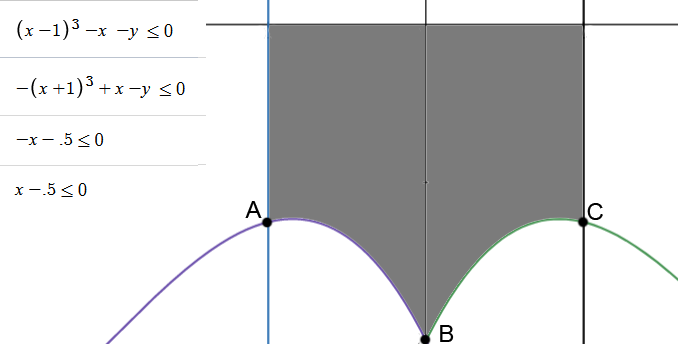
\includegraphics[scale=0.5]{images/Chapter4/constrained optimization example.png}
    \end{center}
    Note the global minimum $B$ and points $A$ and $C$ which lie on the boundary and lead to local minimums outside the boundary. Running projected gradient decent in a neighborhood of $A$ or $C$ will result in getting stuck against the regions boundary.
    \item $L(f) = f + \alpha(x^2 - y^2 - 1)$
    \item $$    L(f) = -x_1 + -x_2 + \alpha_1(x_1 + 2x_2 - 3) + \alpha_2(3x_1 +x_2 - 5) $$
    $$    \frac{\partial L(f)}{\partial x_1} = -1 + \alpha_1 + 3\alpha_2 $$
    $$    \frac{\partial L(f)}{\partial x_2} = -1 + 2\alpha_2 + \alpha_2 $$
    
    solving this linear system yields $\alpha_1 =\frac{2}{5} \alpha_2 = \frac{1}{5}$.
    By the complementary slackness condition of KKT, this gives us
    $x_1 +2x_2 - 3 = 0 $ and $3x_1 + x_2 = 0$.
    solving this linear system yields 
    $x_1 = \frac{11}{5}$ and $x_2 = \frac{-4}{5}$
\end{enumerate}